Este capítulo, correspondiente al objetivo específico 3, presenta el diseño de actividades gamificadas y de las experiencias interactivas que conforman el prototipo orientado a fortalecer las habilidades de aprender a aprender y escucha activa en estudiantes de ingeniería. El contenido se centra en la aplicación práctica de la fundamentación expuesta en la Revisión de Literatura, utilizando dichos lineamientos para definir la estructura de las actividades, seleccionar los recursos educativos apropiados y articular las acciones e interacciones que permiten que cada módulo favorezca el desarrollo de la habilidad que aborda.

\section{Actividades implementadas en el prototipo}

Esta sección describe las actividades implementadas en cada uno de los módulos del prototipo. Su propósito es presentar, de manera clara y estructurada, las acciones que realiza el estudiante dentro de la plataforma y la forma en que cada módulo articula sus funcionalidades para favorecer el desarrollo de las habilidades de aprender a aprender y escucha activa. La descripción de las actividades permite contextualizar el uso de los recursos educativos presentados en la sección siguiente.

\subsection{Actividades implementadas en el módulo aprender a aprender}

El módulo de aprender a aprender organiza sus actividades en torno a la planificación, ejecución y reflexión del proceso de aprendizaje del estudiante. Las actividades implementadas son:

\begin{itemize}

\item \textbf{Creación de roadmaps personalizados:} El estudiante puede generar un plan de aprendizaje mediante dos opciones: (1) una propuesta automática creada por el sistema a partir de sus intereses, conocimientos previos, estilo de aprendizaje y disponibilidad de tiempo, o (2) la construcción manual de un roadmap desde cero mediante el editor visual.

\item \textbf{Edición mediante un editor visual de planes de aprendizaje:} El prototipo incluye un editor gráfico donde el estudiante puede crear, modificar y reorganizar la estructura de su plan de aprendizaje. Este editor permite añadir objetivos, tareas, modificar descripciones, visualizar la relación entre componentes y estructurar el plan de manera clara e intuitiva.

\item \textbf{Conversión entre roadmap y plan accionable:} El sistema permite transformar un roadmap visual en una estructura detallada basada en metas, objetivos y tareas, así como convertir un plan accionable nuevamente en un roadmap editable. Esta función facilita alternar entre una vista general del aprendizaje y una versión operativa del plan, donde cada componente se vuelve ejecutable y rastreable, permitiendo que las tareas avancen por distintos estados (No iniciado, En progreso, En pausa, Completado).

\item \textbf{Exploración de planes de aprendizaje públicos:} El módulo ofrece un espacio para descubrir planes de aprendizaje creados por otros usuarios. El estudiante puede explorar, filtrar por autor o número de pasos, visualizar descripciones y revisar la estructura completa del plan antes de decidir si desea incorporarlo a su propio proceso.

\item \textbf{Copia y reutilización de planes públicos:} A partir de un plan de aprendizaje público, el estudiante puede crear una copia en su cuenta para adaptarlo a sus metas personales. Esta funcionalidad facilita el acceso a modelos de referencia y acelera la planificación inicial.

\item \textbf{Gestión de objetivos y tareas:} Una vez creado el roadmap o copiado un plan existente, el estudiante puede añadir, editar y organizar objetivos y tareas asociadas a sus metas de aprendizaje, estructurando el proceso en pasos concretos y alcanzables.

\item \textbf{Seguimiento del progreso mediante Kanban:} Las tareas asignadas a cada objetivo pueden gestionarse visualmente mediante un tablero Kanban con las columnas “Por hacer”, “En progreso”, “En pausa” y “Completado”, permitiendo al estudiante monitorear su avance y tomar decisiones informadas sobre su proceso.

\item \textbf{Desarrollo de tareas de aprendizaje:} Al seleccionar una tarea, el estudiante accede a su descripción completa y a los recursos asociados que apoyan su realización. El avance de la tarea (como iniciarla, pausarla o completarla) se gestiona mediante el movimiento de la tarjeta correspondiente dentro del tablero Kanban del objetivo.

\item \textbf{Agregación de recursos a las tareas:} Cada tarea admite la incorporación de recursos externos en distintos formatos (videos, artículos, documentos, libros o enlaces web). Esta funcionalidad permite que el estudiante disponga de materiales de apoyo directamente vinculados con la actividad que debe realizar.

\item \textbf{Registro de notas personales por tarea:} El módulo permite añadir notas asociadas a una tarea específica, facilitando que el estudiante registre ideas, recordatorios, reflexiones rápidas o información complementaria relevante para el desarrollo del aprendizaje.

\item \textbf{Autoevaluación y reflexión guiada al finalizar una tarea:} Al completar una tarea, el sistema presenta un conjunto de preguntas orientadas a la reflexión autorregulada. Estas incluyen la intención de aprendizaje, las estrategias utilizadas, las dificultades encontradas, los aspectos logrados y el plan de mejora para futuras actividades; además, el estudiante puede indicar si logró establecer una conexión con conocimientos previos.

\item \textbf{Acceso a reportes de aprendizaje:} El estudiante puede consultar un historial de autoevaluaciones asociadas a todas las tareas completadas. Este apartado permite ordenar y filtrar los reportes según fecha, nivel de dificultad o estado de ánimo, facilitando el análisis de patrones de desempeño y el fortalecimiento del monitoreo metacognitivo.

\item \textbf{Configuración de visibilidad de los planes de aprendizaje:} Cada roadmap puede configurarse como privado o público. En la modalidad pública, el plan puede compartirse mediante un enlace, lo que permite al estudiante controlar quién puede visualizar, copiar o reutilizar sus planes de aprendizaje dentro de la plataforma.

\end{itemize}

\begin{figure}[H]
    \centering
    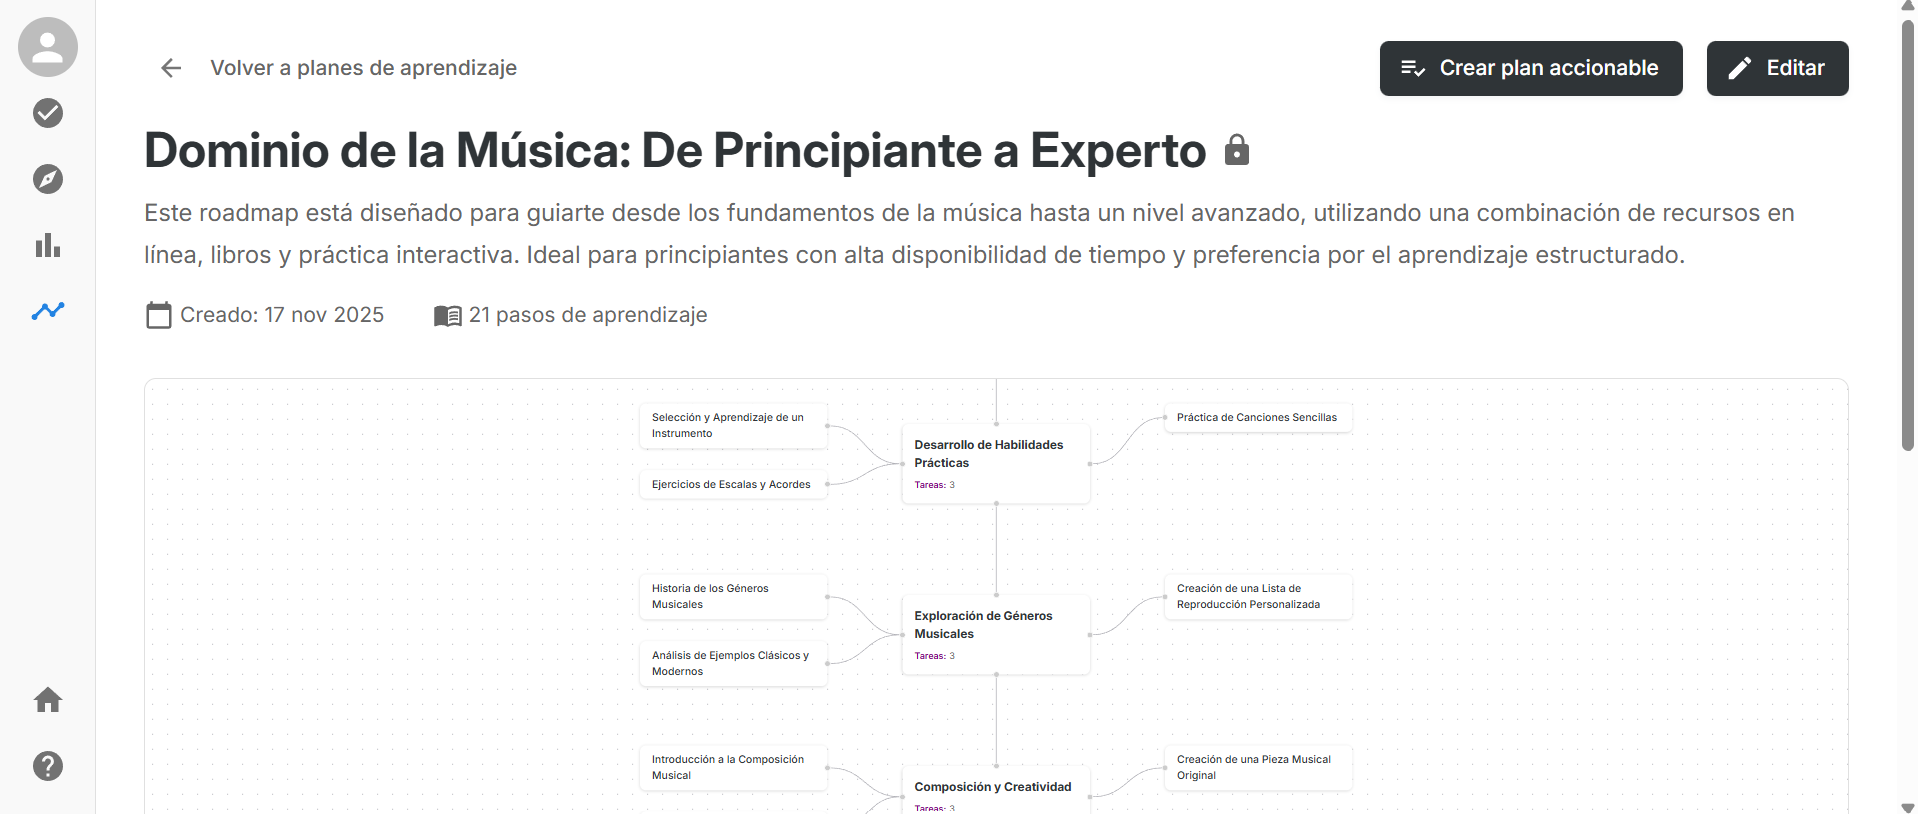
\includegraphics[width=\textwidth]{Figuras/interfaces_AaA/imagen_representativa_modulo_AaA.png}
    \caption{Vista representativa del módulo \textit{Aprender a Aprender}}
    \label{fig:modulo_aprender_a_aprender}
\end{figure}

\noindent Las interfaces que ilustran el funcionamiento de estas actividades se encuentran detalladas en el \hyperref[anexo:interfaces_aprender]{Anexo C}, organizadas en el mismo orden en que se presentan las actividades descritas.


\subsection{Actividades implementadas en el módulo de escucha activa} El módulo de escucha activa está estructurado como un conjunto de rondas de juego, en las que el estudiante interactúa con audios generados automáticamente y ejercicios diseñados para fortalecer habilidades específicas de comprensión auditiva. Las actividades implementadas son:

\begin{itemize}

\item \textbf{Configuración inicial de la sesión de juego:} Antes de comenzar una sesión, el estudiante puede definir parámetros como el número total de rondas, el máximo de repeticiones permitidas por ronda, los tipos de prompts habilitados (descriptivo, evento histórico, instructivo, diálogo, diálogo narrado) y el nivel de dificultad. También puede decidir si desea reutilizar desafíos existentes o generar nuevos contenidos de forma dinámica.

\item \textbf{Inicio de la sesión de juego:} Tras configurar la sesión, el estudiante inicia una experiencia compuesta por una secuencia de rondas. Cada ronda se prepara con un tipo de prompt y un modo de juego específico, de acuerdo con la configuración seleccionada.

\item \textbf{Reproducción del audio:} En cada ronda, el estudiante escucha un clip de audio generado mediante IA, cuyo contenido varía según el tipo de prompt seleccionado. El sistema asegura que cada audio esté alineado con el estilo, dificultad y duración establecidos.

\item \textbf{Resolución del ejercicio según el modo de juego:} Una vez escuchado el audio, el estudiante completa el ejercicio correspondiente al modo de juego asignado: selección múltiple (Focus), completar espacios (Cloze), paráfrasis (Paraphrase), resumen (Summarize) o formulación de preguntas de aclaración (Clarify).

\item \textbf{Manejo de repeticiones de audio por ronda:} Cada ronda permite un número limitado de reproducciones del audio, configurado al iniciar la sesión. El estudiante puede volver a escuchar el clip para reforzar su comprensión antes de responder el ejercicio, siempre dentro del máximo permitido. Las repeticiones aplican únicamente a la escucha del audio, no al envío de la respuesta.

\item \textbf{Envío de respuesta y retroalimentación:} Tras enviar la respuesta, el sistema genera retroalimentación inmediata que incluye la puntuación obtenida, los aciertos, los errores y, en el caso de Clarify, la comparación entre las preguntas formuladas por el estudiante y las preguntas de referencia generadas por el sistema.

\item \textbf{Progresión automática a la siguiente ronda:} Una vez revisada la retroalimentación, el sistema dirige al estudiante a la siguiente ronda. Este proceso continúa hasta completar el total de rondas configuradas.

\item \textbf{Finalización de la sesión:} Al completar todas las rondas, el sistema presenta un resumen global del desempeño de la sesión: número de rondas, puntuación total, respuestas correctas e incorrectas, así como un histórico detallado de cada ronda.

\item \textbf{Revisión detallada de cada ronda:} El estudiante puede acceder a un reporte individual de cada ronda, que incluye el audio utilizado, la respuesta enviada, la puntuación asignada, los intentos realizados y (cuando aplica) la comparación entre sus preguntas y las preguntas de referencia del sistema.

\end{itemize}

\begin{figure}[H]
    \centering
    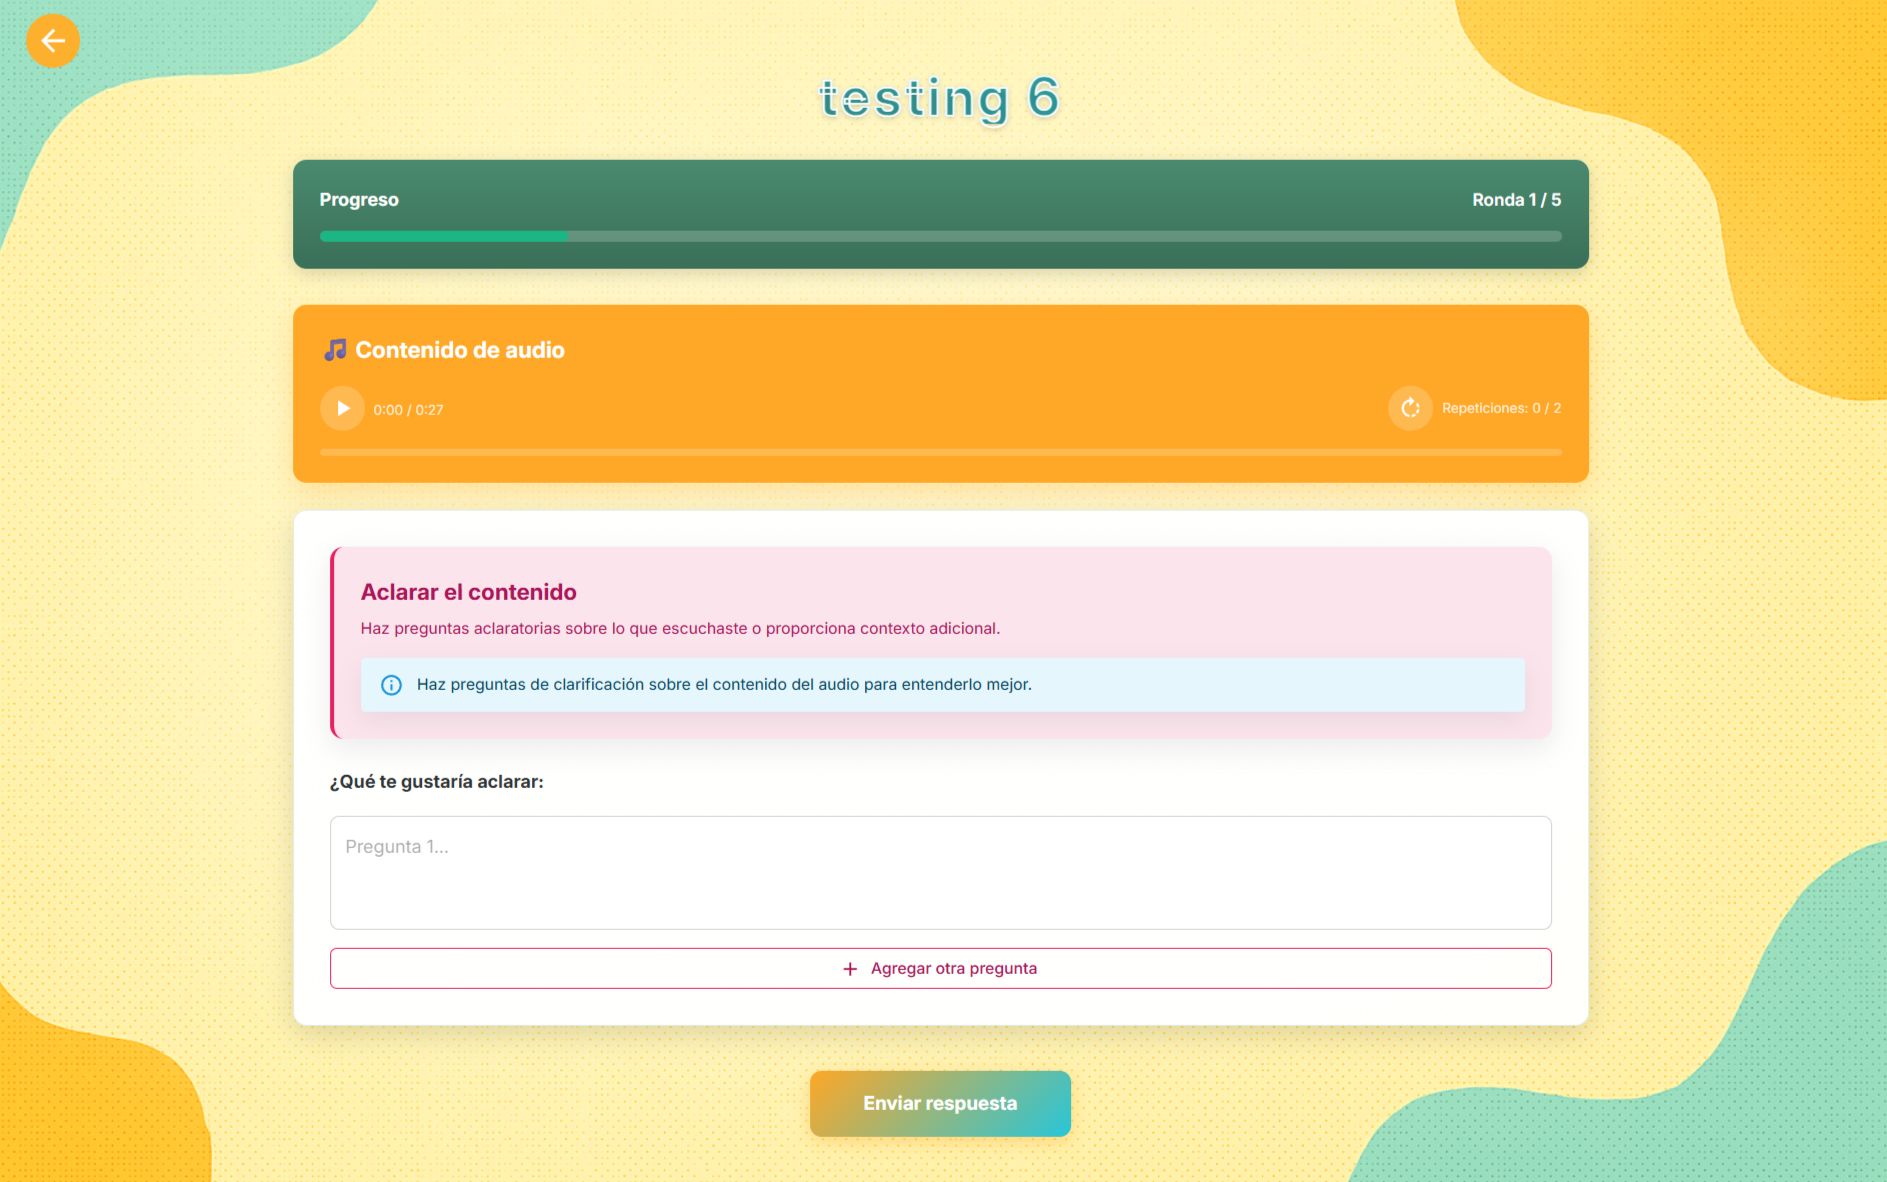
\includegraphics[width=\textwidth]{Figuras/interfaces_EA/ea_ronda_juego.png}
    \caption{Vista representativa del módulo \textit{Escucha activa}}
    \label{fig:modulo_escucha_activa}
\end{figure}

\noindent Las interfaces que ilustran el funcionamiento de estas actividades se encuentran detalladas en el \hyperref[anexo:interfaces_escucha_activa]{Anexo D}, organizadas en el mismo orden en que se presentan las actividades descritas.

\section{Recursos educativos empleados}
Esta sección presenta los recursos educativos empleados en cada uno de los módulos del prototipo. En el contexto de este proyecto, se entiende por recursos educativos a los contenidos, herramientas, apoyos y elementos instruccionales que facilitan el aprendizaje del estudiante y que contribuyen al desarrollo de las habilidades de aprender a aprender y escucha activa.

\subsection{Recursos educativos empleados en el módulo aprender a aprender}
Los recursos educativos integrados en este módulo apoyan al estudiante en la planificación, organización y monitoreo de su propio proceso de aprendizaje:

\begin{itemize}

\item \textbf{Estructura metas–objetivos–tareas:} Organización del proceso de aprendizaje en metas, objetivos y tareas que facilitan la planificación, la priorización y la organización del trabajo personal, fortaleciendo habilidades de autorregulación.

\item \textbf{Roadmaps generados por IA o construidos manualmente:} Planes estructurados de aprendizaje creados a partir de la información ingresada por el estudiante (intereses, conocimientos previos, estilo de aprendizaje y disponibilidad de tiempo), que orientan la planificación inicial y permiten visualizar la secuencia de objetivos y tareas.

\item \textbf{Tablero Kanban:} Herramienta visual que permite al estudiante gestionar el estado de sus tareas a través de columnas como “Por hacer”, “En progreso”, "En pausa", “Completado”, fomentando el monitoreo continuo y la toma de decisiones informada.

\item \textbf{Autoevaluaciones y reflexiones guiadas:} Preguntas y espacios de reflexión que permiten analizar avances, identificar dificultades, evaluar estrategias empleadas y establecer acciones de mejora, fortaleciendo la autorreflexión y el aprendizaje autónomo.

\end{itemize}

\noindent Las interfaces asociadas a estas actividades se encuentran detalladas en el \hyperref[anexo:interfaces_escucha_activa]{Anexo D}, donde se ilustran los distintos momentos de interacción del estudiante durante la sesión de juego, desde su configuración inicial hasta la revisión del desempeño por ronda.



\subsection{Recursos educativos empleados en el módulo de escucha activa}
Los recursos educativos incorporados en este módulo estructuran las actividades de escucha y orientan la interacción del estudiante con los diferentes tipos de ejercicios. A través de estos recursos, el módulo facilita un entrenamiento progresivo de las habilidades vinculadas a la escucha activa.

\begin{itemize}

\item \textbf{Audios generados con IA:} Clips de audio producidos mediante modelos de lenguaje y síntesis de voz, cuyo contenido varía según el tipo de prompt seleccionado (descriptivo, instructivo, diálogo, diálogo narrado, entre otros). Esta variación temática permite ofrecer ejercicios de comprensión auditiva en contextos diversos y más cercanos a situaciones reales.

\item \textbf{Guiones pedagógicos por modo de juego:} Textos adaptados a cada modo de juego (Selección múltiple (Focus), Completar espacios [Cloze], Paráfrasis [Paraphrase], Resumir [Summarize] y Aclarar [Clarify]) que guían al estudiante en habilidades clave de comprensión auditiva, como identificar información relevante, completar contenido, parafrasear, resumir o aclarar ideas.


\item \textbf{Retroalimentación inmediata:} Comentarios automáticos generados al finalizar cada ronda de juego, que permiten al estudiante identificar aciertos, errores y aspectos a mejorar, guiando el proceso de comprensión y fomentando la práctica continua.

\end{itemize}

\section{Elementos de gamificación integrados en el prototipo}
El diseño del prototipo incorpora elementos de gamificación con el fin de aumentar el compromiso, la motivación y la participación del estudiante en las actividades de aprendizaje, tal como lo sugiere la literatura sobre gamificación en entornos digitales. De acuerdo con Watini y Setyowati (2023) \cite{watini2023gamification}, la gamificación consiste en integrar dinámicas, mecánicas y elementos de juego en contextos no lúdicos para promover conductas deseadas, estimular la participación y fortalecer la experiencia del usuario en plataformas de e-learning.
\\
\\
La aplicación de estos principios permite compensar algunas limitaciones propias del aprendizaje en línea, como la falta de interacción emocional presente en entornos presenciales. Desde modelos como el Fogg Behavior Model, la gamificación actúa sobre tres dimensiones clave: motivación, habilidad y disparadores (triggers), favoreciendo estados de alta concentración y participación sostenida durante las actividades educativas.
\\
\\
En coherencia con estos lineamientos, el prototipo integra diversos elementos de gamificación cuidadosamente seleccionados para los módulos de aprender a aprender y escucha activa, con el propósito de fomentar la constancia, facilitar el avance progresivo y aumentar la satisfacción del estudiante durante el uso de la plataforma.

\subsubsection{Elementos de gamificación implementados}

A partir de las recomendaciones presentadas por Watini y Setyowati en su estudio sobre gamificación en entornos de e-learning \cite{watini2023gamification}, se seleccionaron e integraron diversos elementos que refuerzan la motivación, el compromiso y la continuidad en el aprendizaje. La siguiente subsección describe cómo cada uno de estos elementos se materializó en el prototipo desarrollado.

\paragraph{a. Progresión y estructura por niveles}

El prototipo organiza las actividades en etapas claramente definidas (rondas, tareas, objetivos), siguiendo la recomendación de dividir los contenidos en unidades pequeñas que permitan avances graduales y logros frecuentes. Este principio de progresión incremental, señalado por Watini y Setyowati \cite{watini2023gamification}, incrementa la percepción de avance y fortalece la motivación intrínseca.
\\
\\
En el módulo de escucha activa, cada ronda funciona como un “nivel” que se desbloquea al completar la ronda anterior.  
En el módulo aprender a aprender, la estructura metas–objetivos–tareas opera como una jerarquía gamificada de progresión.

\paragraph{b. Recompensas y retroalimentación inmediata}

La retroalimentación instantánea constituye uno de los mecanismos más efectivos para aumentar la motivación en e-learning, al proporcionar claridad sobre el desempeño y reforzar conductas deseadas \cite{watini2023gamification}. El prototipo incorpora este elemento mediante:

\begin{itemize}
    \item Puntuación inmediata al finalizar cada ronda del módulo de escucha activa, diferenciando aciertos, errores y aspectos por mejorar.
    \item Retroalimentación continua en el módulo aprender a aprender mediante autoevaluaciones y la actualización del estado de las tareas en el tablero Kanban.
\end{itemize}

\paragraph{c. Indicadores visuales de progreso}

Según el estudio, los indicadores de progreso (como barras de avance o estados visibles) son efectivos para mantener la motivación al permitir al estudiante monitorear su trayectoria y visualizar cuánto ha completado \cite{watini2023gamification}. En el prototipo se implementaron:

\begin{itemize}
    \item Barra de progreso asociada a cada ronda del módulo de escucha activa.
    \item Estados del Kanban: \textit{Por hacer}, \textit{En progreso}, \textit{En pausa}, \textit{Completado}.
    \item Resúmenes de desempeño al finalizar las sesiones de escucha activa.
\end{itemize}

\paragraph{d. Desafíos y dificultad ajustada}

El artículo enfatiza que los retos deben estar equilibrados para mantener el interés sin generar frustración \cite{watini2023gamification}. Atendiendo a esta recomendación, el prototipo incorpora ajustes dinámicos de dificultad:

\begin{itemize}
    \item En escucha activa, el estudiante puede configurar el nivel de dificultad, lo que ajusta parámetros como la duración del audio, la complejidad semántica y las exigencias del modo de juego.
    \item En aprender a aprender, la dificultad se ve reflejada en la complejidad de las tareas y del proceso de planificación.
\end{itemize}

\paragraph{e. Personalización y sentido de agencia}

Permitir al usuario tomar decisiones dentro del sistema aumenta el sentido de control y, por tanto, la motivación intrínseca \cite{watini2023gamification}. En el prototipo se adoptó este principio mediante:

\begin{itemize}
    \item Configuración personalizada de sesiones: dificultad, tipos de prompt, número de rondas, reutilización de desafíos.
    \item Creación, edición y adaptación de planes de aprendizaje propios.
    \item Copia y personalización de planes públicos para ajustarlos a metas individuales.
\end{itemize}

\paragraph{f. Anticipación y preparación del siguiente paso}

Watini y Setyowati resaltan que la anticipación de la siguiente actividad reduce el abandono y mantiene al usuario dentro del flujo de aprendizaje \cite{watini2023gamification}. El prototipo incorpora este principio mediante:

\begin{itemize}
    \item Transición automática entre rondas en escucha activa.
    \item Indicaciones claras sobre la siguiente tarea, objetivo o ronda a completar.
    \item Resúmenes finales que orientan sobre el desempeño y los pasos siguientes.
\end{itemize}

\paragraph{g. Socialización indirecta como motivador}

Aunque sin competencia directa, el prototipo integra un componente de socialización indirecta, coherente con los principios de comunidad y reconocimiento mencionados por el artículo \cite{watini2023gamification}. Este elemento se expresa mediante:

\begin{itemize}
    \item Exploración de planes de aprendizaje públicos creados por otros estudiantes.
    \item Acceso a estructuras y estrategias ajenas que sirven como inspiración y validación social.
\end{itemize}

Como consolidación de los elementos de gamificación descritos y su relación con los módulos desarrollados, en el \hyperref[anexo:gamificacion]{Anexo E} se presenta una tabla comparativa que resume su implementación en el prototipo.